\documentclass[journal]{IEEEtran}

\usepackage{cite}

\usepackage{amsmath,amssymb,amsfonts}
\usepackage{algorithmic}
\usepackage{graphicx}
\usepackage{textcomp}
\usepackage{xcolor}
\usepackage{booktabs}
\usepackage{multirow}
\usepackage{array}
\usepackage{subfig}
\def\BibTeX{{\rm B\kern-.05em{\sc i\kern-.025em b}\kern-.08em
    T\kern-.1667em\lower.7ex\hbox{E}\kern-.125emX}}

\begin{document}

\title{Distributed Collapsed Gibbs Sampling for LDA on Spark}

\author{\IEEEauthorblockN{Agnieszka Ciborowska}\\
\IEEEauthorblockA{\textit{Department of Computer Science} \\
\textit{Virginia Commonwealth University}}}


\maketitle

\begin{abstract}
The report describes a collapsed Gibbs sampling method for widely-used latent Dirichlet allocation (LDA) model on Spark.
\end{abstract}

% Note that keywords are not normally used for peerreview papers.
\begin{IEEEkeywords}
Spark, LDA, collapsed Gibbs sampling
\end{IEEEkeywords}


\section{Introduction}
Information hidden in very large datasets, such as document texts or images, has became a rapidly growing interest of researches as it provides ability to...

The latent Dirichlet allocation model, proposed by Blei et al.~\cite{blei2003latent}, is a three-level hierarchical Bayesian model designed to discover latent topics in document corpora. The main idea of the model is to represent each document as a random mixture of topics, where each topic is, in turn, modeled by a distribution over words. 

\section{Latent Dirichlet Allocation}
Before describing the detail of the distributed LDA model, I briefly review the standard LDA model, illustrated LDA models each of $D$ documents as a mixture over $K$ latent topics, where each topic is a multinomial probability distribution over a vocabulary of $V$ words. Generative process of creating a new document $j$ can be characterized as follows:
\begin{itemize}
\item draw a mixing proportion $\theta_{k|j}$ from a Dirichlet with parameter $\alpha$,
\item for the $i^{th}$ word in the document, first draw a topic assignment $z_{ij}$, where topic $k$ is chosen with probability of $\theta_{k|j}$, and then value $w$ of word $x_{ij}$ is drawn from the $z_{ij}$ topic with probability $\phi_{w|k}$, where $\phi_{w|z_{ij}}$ is drown from a Dirichlet prior with parameter $\beta$.
\end{itemize}
The above description of the generative process is equivalent to:
$$
\theta_{k|j}\sim Dir(\alpha) \quad \phi_{w|k}\sim Dir(\beta) \quad  z_{ij}\sim \theta_{k|j} \quad  x_{ij}\sim \phi_{w|z_{ij}}
$$
where $\alpha$ and $\beta$ are fixed Dirichlet priors. The graphical representation of the LDA model is presented on Figure~\ref{fig:lda}.
\begin{figure}
\centering
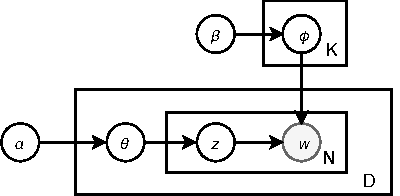
\includegraphics[scale=0.9]{plots/LDA.pdf}
\caption{Graphical model for LDA. Observed variable $w$ is shaded.}
\label{fig:lda}
\end{figure}

Given the observed words $\texttt{x}=x_{ij}$, the task is to compute the posterior distribution over the latent variables $\texttt{z}$, $\theta$ and $\phi$. An accurate inference procedure, proposed by Griffiths and Steyvers\cite{griffiths2004finding}, is a collapsed Gibbs sampling, which samples the latent variable $\texttt{z}$ with $\theta$ and $\phi$ integrated out, what allows to increase the convergence rate. The conditional probability of $z_{ij}$ is given by:
$$
p(z_{ij}=k|z^{\lnot ij}, x, \alpha, \beta) = \dfrac{c_{k,m,\cdot} + \alpha}{N_{j}^{\lnot i}+K\alpha} \frac{c_{k,\cdot,n} + \beta}{c_{k,\cdot,\cdot} + V\beta}
$$ 
where $\lnot ij$ denotes word $i$ in document $j$ that is excluded in the count values and $c_{k,m,n}$ represents the number of times topic $k$ is assigned to word $n$ in document $m$. Missing index value for $c_{k,m,n}$ (e.g. $c_{k,\cdot,n}$) denotes summing over the index (e.g. $c_{k,\cdot,n} = \sum_{m=1}^{M} c_{k,m,n}$.

\section{Distributed inference for LDA}

\begin{figure*}[t]
\centering
\subfloat[ABC news headlines dataset.]{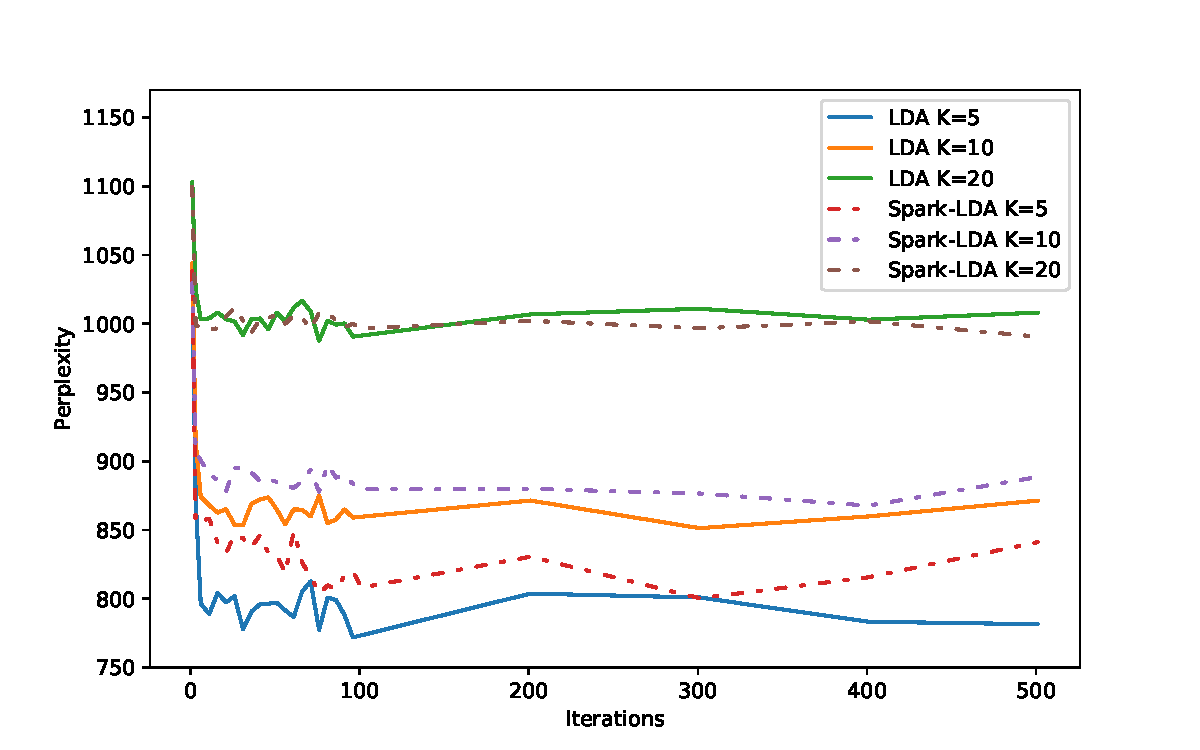
\includegraphics[scale=0.4]{plots/perplexity1.pdf}%
\label{fig:perplex2}}
\hfil
\subfloat[NIPS abstracts dataset.]{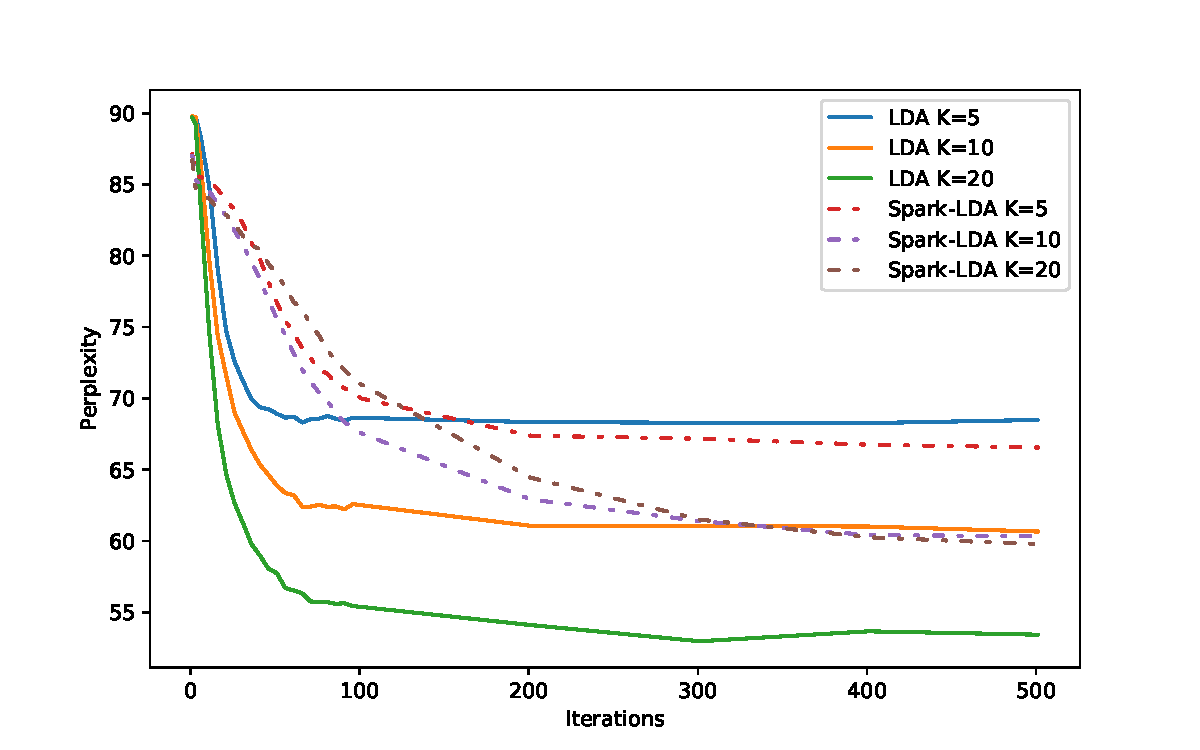
\includegraphics[scale=0.4]{plots/perplexity2.pdf}%
\label{fig:perplex2}}
\caption{Perplexity during training for different number of topics.}
\label{fig_sim}
\end{figure*}

\renewcommand{\arraystretch}{1.3}

\begin{table*}[t]
\centering
\caption{Speedup of Spark-LDA on ABC News headlines (short) and NIPS abstracts datasets with respect to different number of topics.}
\begin{tabular}{lrrrrrrr} \toprule
                 & \multicolumn{3}{c}{\textbf{ABC News headlines}} & \multicolumn{3}{c}{\textbf{NIPS abstracts}}        & \multicolumn{1}{c}{\textbf{ABC News headlines (full)}} \\
                 & K = 5             & K = 10           & K = 20           & K = 5           & K = 10          & K = 20         & K = 2                                           \\ \midrule
LDA              & 47,80             & 51,59            & 57,41            & 1 729,06        & 1 779,65        & 2 002,13       & 32 577,60                                       \\
Spark-LDA        & 117,27            & 126,82           & 143,06           & 128,03          & 159,32          & 207,01         & 3 929,08                                        \\ \midrule
\textbf{Speedup} & \textbf{0,408}    & \textbf{0,407}   & \textbf{0,401}   & \textbf{13,505} & \textbf{11,170} & \textbf{9,672} & \textbf{8,291}  \\ \bottomrule                         
\end{tabular}
\label{tab:speedup}
\end{table*}

\begin{figure*}[t]
\centering
\subfloat[ABC News headlines dataset.]{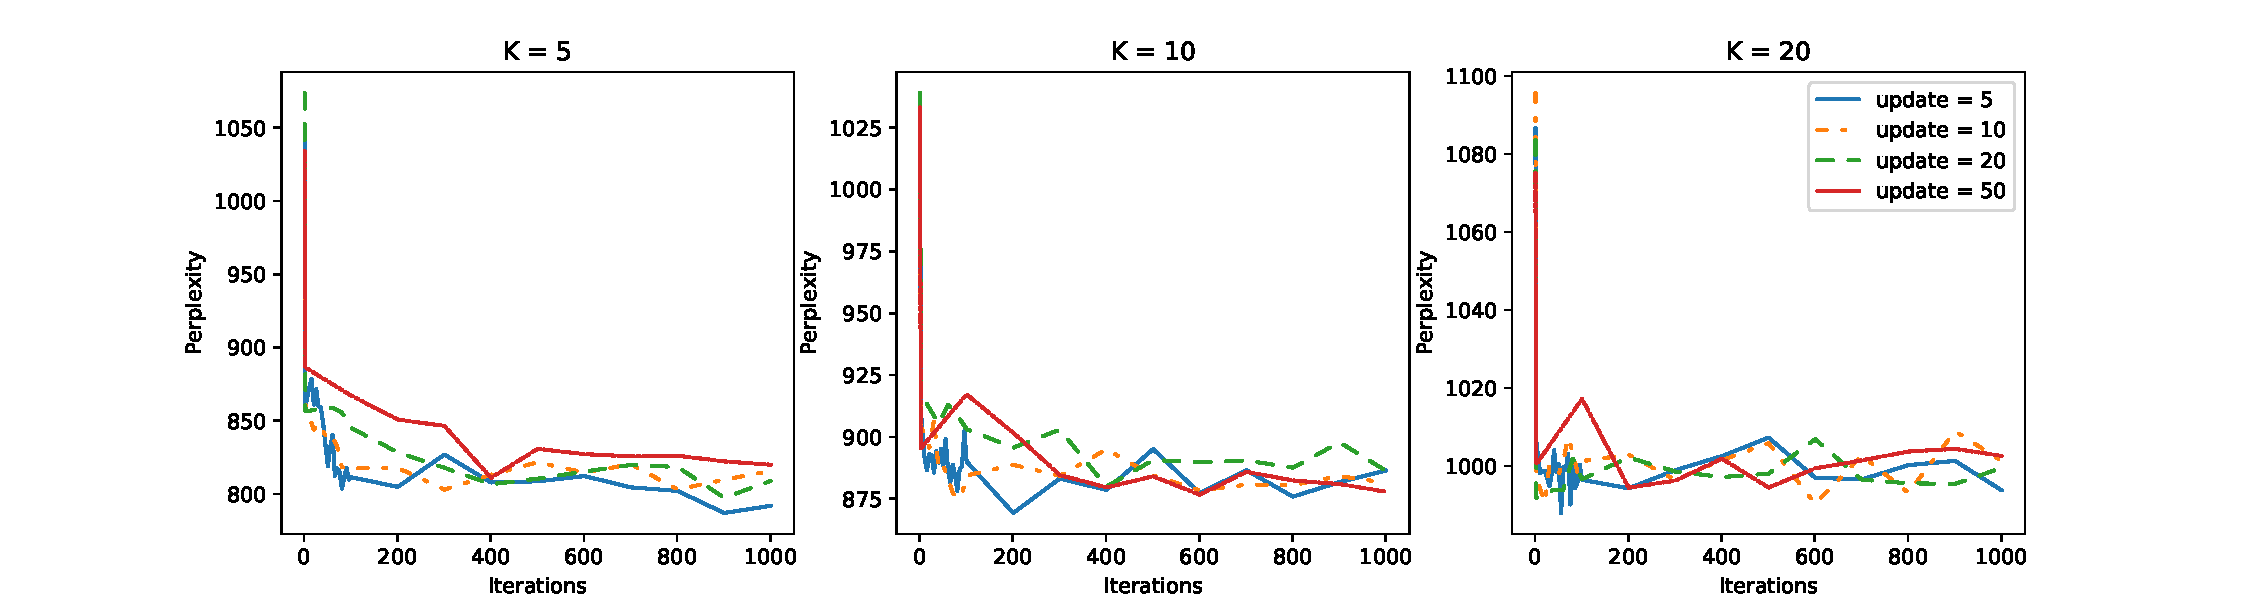
\includegraphics[scale=0.4]{plots/update_abc.pdf}%
\label{fig:param_abc}}
\hfil
\subfloat[NIPS abstracts dataset.]{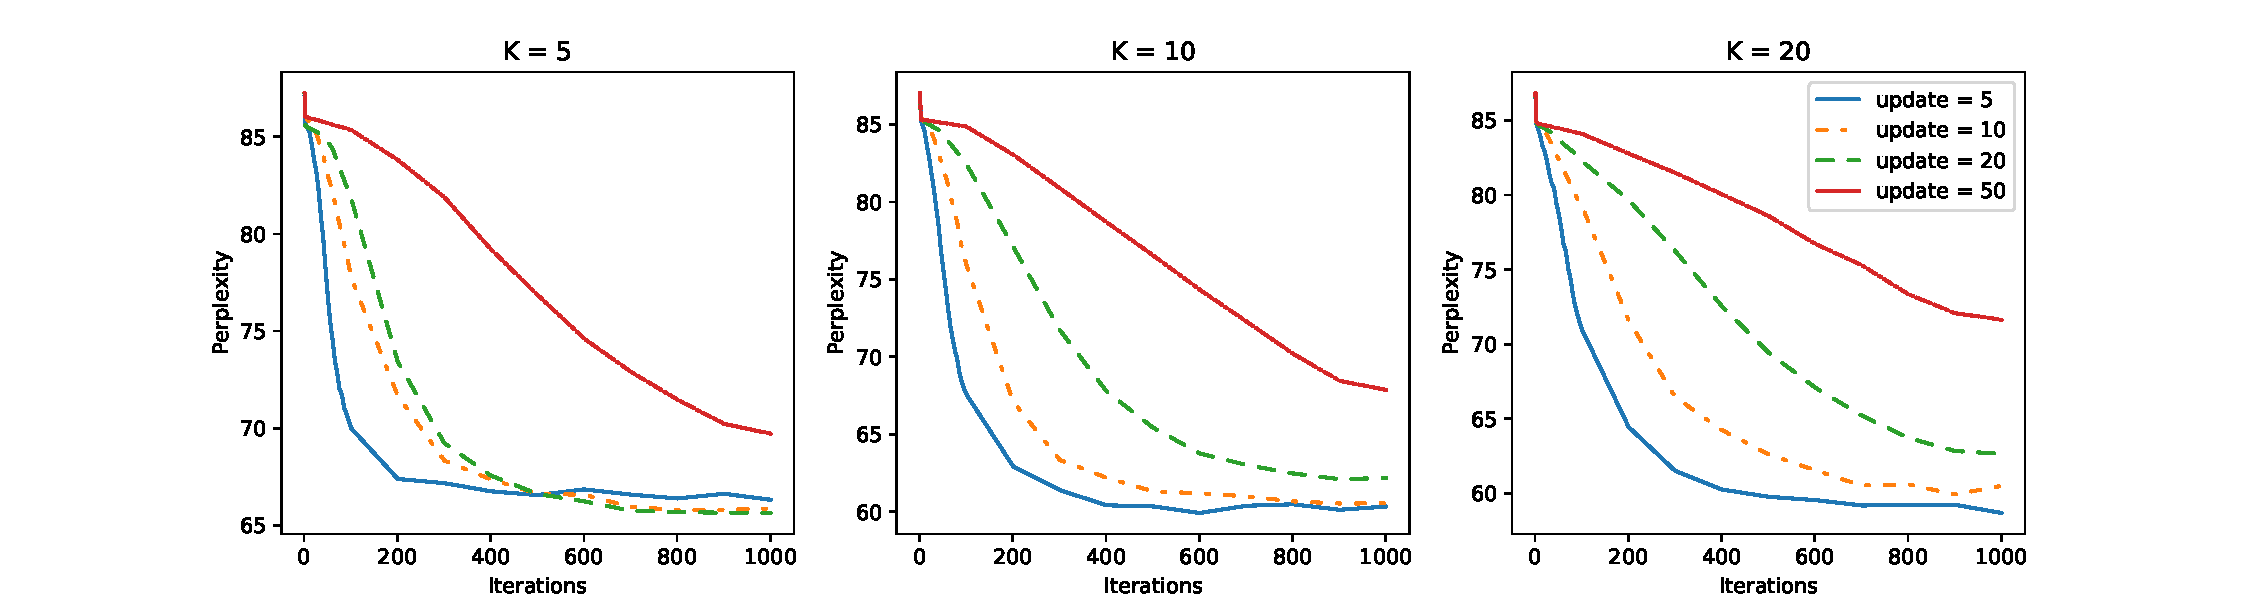
\includegraphics[scale=0.4]{plots/update_abstract.pdf}%
\label{fig:param_nips}}
\caption{Perplexity during training Spark-LDA for different interval between parameter updates .}
\label{fig_sim}
\end{figure*}

\begin{figure*}[t]
\centering
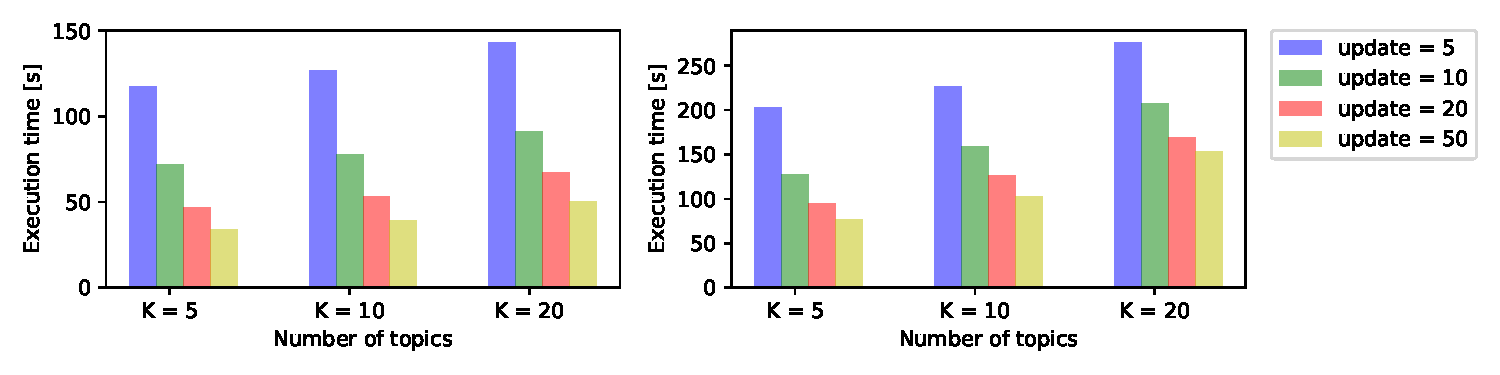
\includegraphics[scale=0.7]{plots/param_update.pdf}
\caption{Execution time of Spark-LDA on ABC News headlines (left) and NIPS abstracts (right) with respect to interval between global parameters update.}
\label{fig_sim}
\end{figure*}



\section{Conclusion}
The conclusion goes here.

\bibliographystyle{IEEEtran}
\bibliography{IEEEabrv,paper}

%\vfill

% Can be used to pull up biographies so that the bottom of the last one
% is flush with the other column.
%\enlargethispage{-5in}



% that's all folks
\end{document}


